% !TEX TS-program = pdflatex
% !TEX encoding = UTF-8 Unicode

% This is a simple template for a LaTeX document using the "article" class.
% See "book", "report", "letter" for other types of document.

\documentclass[11pt]{article} % use larger type; default would be 10pt

\usepackage[utf8]{inputenc} % set input encoding (not needed with XeLaTeX)
\usepackage{braket}
%%% Examples of Article customizations
% These packages are optional, depending whether you want the features they provide.
% See the LaTeX Companion or other references for full information.
\usepackage{placeins}
%%% PAGE DIMENSIONS
\usepackage{geometry} % to change the page dimensions
\geometry{a4paper} % or letterpaper (US) or a5paper or....
% \geometry{margin=2in} % for example, change the margins to 2 inches all round
% \geometry{landscape} % set up the page for landscape
%   read geometry.pdf for detailed page layout information

\usepackage{graphicx} % support the \includegraphics command and options

% \usepackage[parfill]{parskip} % Activate to begin paragraphs with an empty line rather than an indent

%%% PACKAGES
\usepackage{booktabs} % for much better looking tables
\usepackage{array} % for better arrays (eg matrices) in maths
\usepackage{paralist} % very flexible & customisable lists (eg. enumerate/itemize, etc.)
\usepackage{verbatim} % adds environment for commenting out blocks of text & for better verbatim
\usepackage{subfig} % make it possible to include more than one captioned figure/table in a single float
% These packages are all incorporated in the memoir class to one degree or another...

%%% HEADERS & FOOTERS
\usepackage{fancyhdr} % This should be set AFTER setting up the page geometry
\pagestyle{fancy} % options: empty , plain , fancy
\renewcommand{\headrulewidth}{0pt} % customise the layout...
\lhead{}\chead{}\rhead{}
\lfoot{}\cfoot{\thepage}\rfoot{}

%%% SECTION TITLE APPEARANCE
\usepackage{sectsty}
\allsectionsfont{\sffamily\mdseries\upshape} % (See the fntguide.pdf for font help)
% (This matches ConTeXt defaults)

%%% ToC (table of contents) APPEARANCE
\usepackage[nottoc,notlof,notlot]{tocbibind} % Put the bibliography in the ToC
\usepackage[titles,subfigure]{tocloft} % Alter the style of the Table of Contents
\renewcommand{\cftsecfont}{\rmfamily\mdseries\upshape}
\renewcommand{\cftsecpagefont}{\rmfamily\mdseries\upshape} % No bold!

%%% END Article customizations

%%% The "real" document content comes below...

\title{Nuclear Structure Assignment 4}
\author{Charles Loelius}
%\date{} % Activate to display a given date or no date (if empty),
         % otherwise the current date is printed 

\begin{document}
\maketitle

\section{Exercise 9}

In this case we want to make a table of all possible partial waves with isospin T, projection $T_z$, spin S, orbital momentum L and total spin J.  We limit the cases to J$\leq$ 2.

\begin{table}[hbt!]
\centering
\begin{tabular}{|c|c|c|c|c|c|}
 Isospin(T) & Projection ($T_z$) & Spin(S) & Orbital (L) & Total Spin(J)& Spectroscopic Notation\\
\hline
$\frac{1}{2}$ & $\frac{1}{2}$& $\frac{1}{2}$ & 0 &$ \frac{1}{2}$ & $^{2}S_{\frac{1}{2}}$\\

$\frac{1}{2}$ & $\frac{1}{2}$& $\frac{1}{2}$ & 1 &$ \frac{1}{2}$ & $^{2}P_{\frac{1}{2}}$\\

$\frac{1}{2}$ & $\frac{1}{2}$& $\frac{1}{2}$ & 1 &$ \frac{3}{2}$ & $^{2}P_{\frac{3}{2}}$\\
$\frac{1}{2}$ & $\frac{1}{2}$& $\frac{1}{2}$ & 2 &$ \frac{3}{2}$ & $^{2}D_{\frac{3}{2}}$\\
$\frac{1}{2}$ & $\frac{1}{2}$& $\frac{1}{2}$ & 2 &$ \frac{5}{2}$ & $^{2}D_{\frac{5}{2}}$\\
$\frac{1}{2}$ & $-\frac{1}{2}$& $\frac{1}{2}$ & 0 &$ \frac{1}{2}$ & $^{2}S_{\frac{1}{2}}$\\

$\frac{1}{2}$ & $-\frac{1}{2}$& $\frac{1}{2}$ & 1 &$ \frac{1}{2}$ & $^{2}P_{\frac{1}{2}}$\\

$\frac{1}{2}$ & $-\frac{1}{2}$& $\frac{1}{2}$ & 1 &$ \frac{3}{2}$ & $^{2}P_{\frac{3}{2}}$\\
$\frac{1}{2}$ & $-\frac{1}{2}$& $\frac{1}{2}$ & 2 &$ \frac{3}{2}$ & $^{2}D_{\frac{3}{2}}$\\
$\frac{1}{2}$ & $-\frac{1}{2}$& $\frac{1}{2}$ & 2 &$ \frac{5}{2}$ & $^{2}D_{\frac{5}{2}}$\\
\hline
1 & 1 & 0 & 0 & 0 & $^{1}S_0$\\
1 & 1 & 0 & 1 & 1 & $^{1}P_1$\\
1 & 1 & 0 & 2 & 2 & $^{1}D_2$\\
1 & 0 & 0 & 0 & 0 & $^{1}S_0$\\
1 & 0 & 0 & 1 & 1 & $^{1}P_1$\\
1 & 0 & 0 & 2 & 2 & $^{1}D_2$\\
1 & 0 & 1 & 0 & 0 & $^{3}S_1$\\
1 & 0 & 1 & 1 & 0 & $^{3}P_0$\\
1 & 0 & 1 & 1 & 1 & $^{3}P_1$\\
1 & 0 & 1 & 1 & 2 & $^{3}P_2$\\
1 & 0 & 1 & 2 & 1 & $^{3}D_1$\\
1 & 0 & 1 & 2 & 2 & $^{3}D_2$\\
1 & 0 & 1 & 2 & 3 & $^{3}D_3$\\
1 & -1 & 0 & 0 & 0 & $^{1}S_0$\\
1 & -1 & 0 & 1 & 1 & $^{1}P_1$\\
1 & -1 & 0 & 2 & 2 & $^{1}D_2$\\
\hline
$\frac{3}{2}$ & $\frac{1}{2}$& $\frac{1}{2}$ & 0 &$ \frac{1}{2}$ & $^{2}S_{\frac{1}{2}}$\\

$\frac{3}{2}$ & $\frac{1}{2}$& $\frac{1}{2}$ & 1 &$ \frac{1}{2}$ & $^{2}P_{\frac{1}{2}}$\\

$\frac{3}{2}$ & $\frac{1}{2}$& $\frac{1}{2}$ & 1 &$ \frac{3}{2}$ & $^{2}P_{\frac{3}{2}}$\\
$\frac{3}{2}$ & $\frac{1}{2}$& $\frac{1}{2}$ & 2 &$ \frac{3}{2}$ & $^{2}D_{\frac{3}{2}}$\\
$\frac{3}{2}$ & $\frac{1}{2}$& $\frac{1}{2}$ & 2 &$ \frac{5}{2}$ & $^{2}D_{\frac{5}{2}}$\\
$\frac{3}{2}$ & $-\frac{1}{2}$& $\frac{1}{2}$ & 0 &$ \frac{1}{2}$ & $^{2}S_{\frac{1}{2}}$\\

$\frac{3}{2}$ & $-\frac{1}{2}$& $\frac{1}{2}$ & 1 &$ \frac{1}{2}$ & $^{2}P_{\frac{1}{2}}$\\

$\frac{3}{2}$ & $-\frac{1}{2}$& $\frac{1}{2}$ & 1 &$ \frac{3}{2}$ & $^{2}P_{\frac{3}{2}}$\\
$\frac{3}{2}$ & $-\frac{1}{2}$& $\frac{1}{2}$ & 2 &$ \frac{3}{2}$ & $^{2}D_{\frac{3}{2}}$\\
$\frac{3}{2}$ & $-\frac{1}{2}$& $\frac{1}{2}$ & 2 &$ \frac{5}{2}$ & $^{2}D_{\frac{5}{2}}$\\

\hline
\end{tabular}
\caption{Table of Allowed Partial Waves}
\end{table}
\FloatBarrier
Here the table includes all possible $l,j$ states less than j=2 for the case where there is one particle (Isospin=$\frac{1}{2}$). Now in the case of two particles, $T=1$. If the projection is $\pm 1$ we cannot have both spins the same, which limits the total spin to zero. However if they are different particles then $T_z=0$ and any spin combination is possible. This explains the much larger number of possible states for $T_z=0$.\\

However, in the case of three particles there is only one form the system can take, namely that two particles are of one isospin projection and the other is different. This leads to the two that are the same having the opposite spin(and so canceling out their spin effects). Thus the only degrees of freedom are in which isospin has two particles, and the angular momentum l.

\section{Exercise 10: Spin Orbit Force}

We note that here the spin orbit force becomes \\

\begin{equation} U_{so}=A S \cdot L \end{equation}

We then note that\\

\begin{equation}
J^2=(L+S)^2=L^2+S^2+2L\cdot S
\end{equation}

Now we then note that if we take the expectation value we have\\

\begin{equation}
\braket{J^2}=\braket{L^2}+\braket{S^2}+2\braket{L\cdot S}
\end{equation}

Hence we have that\\

\begin{equation}
\braket{L \cdot S}=\frac{J(J+1)-L(L+1)-S(S+1)}{2}\end{equation}

And so we have that\\
\begin{equation}
U_{so}=\frac{A}{2}\left(J(J+1)-L(L+1)-S(S+1)\right)\end{equation}
\subsection{S waves have no spin-orbit force}

Now we then note that if $L=0$ it follows that $J=S$ and so
\begin{equation}
U_{so}=\frac{A}{2}\left(J(J+1)-L(L+1)-S(S+1)\right)=\frac{A}{2}\left(J(J+1)-J(J+1)\right)=0\end{equation}

The same holds for the spin singlet states where $S=0$, as is reasoanble.\\

\subsection{Expectation value of pauli matricies}
\begin{equation}
\braket{\sigma_1 \cdot \sigma_2}=\frac{1}{2}\left((\sigma_1+\sigma_2)^2-\braket{\sigma_1^2}-\braket{\sigma_2}^2\right)
=\frac{1}{2} \left(\braket{(\sigma_1+\sigma_2)^2}-6\right)
\end{equation}

Here we have done the same as before with the sum, and have noted that $\vec{\sigma}=\braket{\sigma_1,\sigma_2,\sigma_3}$ . We then note that $\sigma_i \cdot \sigma_i =I$, and so $\vec{\sigma}\cdot \vec{\sigma}=3$

\subsection{All cases for $\braket{\sigma_1 \cdot \sigma_2 \tau_1 \cdot \tau_2}$}

We begin by noting that S=0 implies $\braket{(\sigma_1+\sigma_2)^2}=0$ and $S=1$ implies $\braket{(\sigma_1+\sigma_2)^2}=8=2^2*1(1+1)$ and the same is true for the $\tau$ matricies(assuming spin one half particles).\\

We can thus make a table of the values of this product as\\
\FloatBarrier
\begin{table}[bht!]
\centering
\begin{tabular}{c|c|c}
$\sigma$ & $\tau$ & $\braket{\sigma_1 \cdot \sigma_2 \tau_1 \cdot \tau_2}$\\
0 & 0 & 9\\
0 & 1 & -3\\
1 & 0 & -3\\
1 &1 &1
\end{tabular}
\end{table}
\section{Exercise 11}

We now consider the V8 potential model with\\

\begin{equation}
V(r)=\left(C_C^0+C_C^1+C_\sigma \sigma_1 \cdot \sigma_2 + C_T \left( 1+\frac{3}{m_\alpha r} +\frac{3}{(m_\alpha r)^2}\right) S_{12}(\hat{r})+C_{SL}\left(\frac{1}{m_\alpha r}+\frac{1}{(m_\alpha r)^2}\right) L\cdot S\right) \frac{e^{-m_\alpha r}}{m_\alpha r}
\end{equation}


Now we then consider ony the one pion exchange term. This is:\\

\begin{equation}
V(r)=\frac{-f_\pi^2}{4\pi m_\pi^2 }\frac{\tau_1 \cdot \tau_2}{3}\left( \sigma_1 \cdot \sigma_2 +  \left( 1+\frac{3}{m_\alpha r} +\frac{3}{(m_\alpha r)^2}\right) S_{12}(\hat{r})\right)  \frac{e^{-m_\alpha r}}{m_\alpha r}
\end{equation}

Now we can expand the table from previously to see what the effects are on the different states we found were possible. Obviously in this case we consider only the two particle states.\\

\begin{table}[hbt!]
\centering
\caption{Table of expectation values}
\begin{tabular}{c|c|c|c}
Partial Wave & $\braket{\sigma_1 \cdot \sigma_2}$ & $\braket{\tau_1 \cdot \tau_2}$ & $ \braket{S_{12}}$ \\
$^1 S_0$ & -3 & 1 & 0 \\
$^1 P_1 $& -3 & 1 & 0\\
$^1 D_2$ & -3 & 1 & 0\\
$^1 S_0$ & -3 & -3 & 0\\
$^1 P_1 $& -3 & -3 & 0\\
$^1 D_2 $& -3 & -3 & 0\\
$^3 S_1 $& 1 & -3 & 0\\
$^3 P_0 $& 1 & -3 & 0\\
$^3 P_1 $& 1 & -3 & 2\\
$^3 P_2 $& 1 & -3 &$\frac{-2}{5} $\\
$^3 D_1 $& 1 & -3 &$ -\frac{16}{5}$\\
$^3 D_2 $& 1 & -3 & 2\\
$^3 D_3 $& 1 & -3 & $-\frac{4}{7}$\\

\end{tabular}

\end{table}

The most salient features of this table are two fold. The first is the fact that for any of the isospin =1 cases there is no tensor force and the spin spin force is strongly negative, while the isospin force is somewhat positive. Their product is thus negative, and this is what enters into the force equation. However for the isospin antisymmetric cases, the cases where the spins are not alligned leads to the spin spin and isospin force with a product of $-3 \times -3=9$, but no spin orbit. Finally for the caases where the spins are alligned but the isospin projections are 0, we have in the case where the total spin is equal to the orbital angular momentum an additional spin tensor force that opposes the spin spin force, and in all other cases where $L\neq J$ an additional negative term. \\

\subsection{Dueteron Binding Energy}

The deuteron's ground state is a mixture of the $^{3}S_1$ state  and the $^{3}D_1$ state. We see then that we can construct a graph based on the fact that\\

\begin{equation}
V_{\sigma \cdot \sigma}\approx - \braket{\tau_1 \cdot \tau_2} \braket{\sigma_1 \cdot \sigma_2}\end{equation}

\begin{equation}
V_{S_{12}}\approx -\braket{\tau_1 \cdot \tau_2} \left(1+\frac{3}{x}+\frac{3}{x^2}\right) \braket{S_{12}}
\end{equation}

Where $x=m_\pi r$.

We thus get a relative strength of the tensor force to the spin spin force as a function of x as:\\

\begin{equation}
\frac{V_{S_{12}}}{V_{\sigma \cdot \sigma}}=\frac{\left(1+\frac{3}{x}+\frac{3}{x^2}\right) \braket{S_{12}}}{\braket{\sigma_1 \cdot \sigma_2}}\end{equation}

From the information in the table we see this becomes\\

\begin{equation}
\frac{V_{S_{12}}}{V_{\sigma \cdot \sigma}}=-\frac{\left(1+\frac{3}{x}+\frac{3}{x^2}\right)\frac{-16}{5}}{1}\end{equation}

I plot this below:\\
\begin{figure}[hbt!]
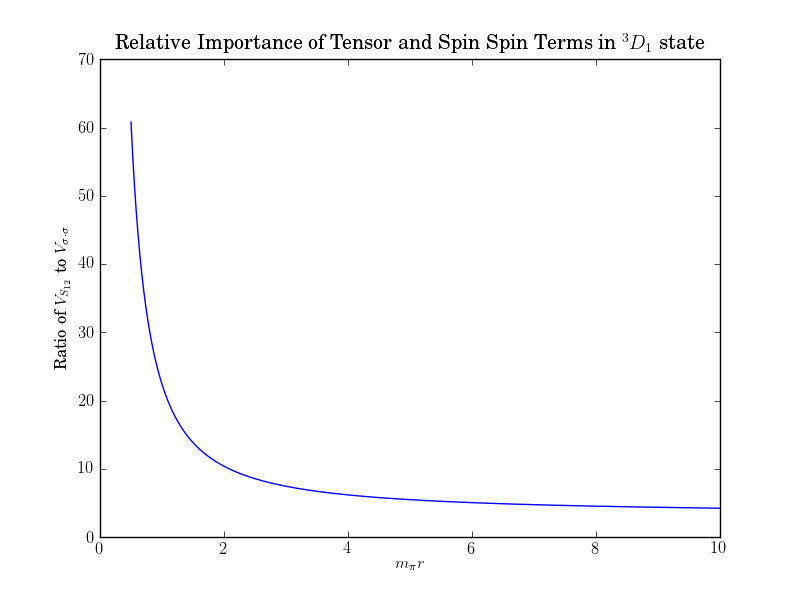
\includegraphics[width=\linewidth]{ratio}
\caption{Comparison of terms}
\end{figure}

We note that the spin spin force and tensor force are of the same sign, and that no matter what the value of x the tensor force is larger than the spin spin sforce. We also see that as the pion approaches masslessness the tensor force becomes infinitely larger, while the spin spin force remains unchanged.

\end{document}
